%%%%%%%%%%%%%%%%%%%%%%%%%%%%%%%%%%%%%%%%%%%%%%%%%%%%%%%%%%%%%%%%%%%%%%%%%%%%%%%%
%2345678901234567890123456789012345678901234567890123456789012345678901234567890
%        1         2         3         4         5         6         7         8

\documentclass[letterpaper, 12 pt, conference]{ieeeconf}  % Comment this line out
                                                          % if you need a4paper
%\documentclass[a4paper, 10pt, conference]{ieeeconf}      % Use this line for a4
                                                          % paper

\IEEEoverridecommandlockouts                              % This command is only
                                                          % needed if you want to
                                                          % use the \thanks command
\overrideIEEEmargins
% See the \addtolength command later in the file to balance the column lengths
% on the last page of the document



% The following packages can be found on http:\\www.ctan.org
\usepackage{graphics} % for pdf, bitmapped graphics files
\usepackage{graphicx} % for scaling graphics files
%\usepackage{epsfig} % for postscript graphics files
%\usepackage{mathptmx} % assumes new font selection scheme installed
% \usepackage{times} % assumes new font selection scheme installed
\usepackage{amsmath} % assumes amsmath package installed
\usepackage{amssymb}  % assumes amsmath package installed
\usepackage{tabularx, array, multirow, booktabs, makecell} % for table formatting
\newcolumntype{C}{>{\centering\arraybackslash}X} % C: center version of X
\usepackage{cuted}   % for overwide graphs
\usepackage{float}   % for table placement

\title{\LARGE \bf
Determining Vacancy in Buildings via Machine Learning Methods
}

\author{Benjamen Neduva, Calvin Cramer, Lionel Quiambao, Lisa M. Slaughter, \\
        Maksim Nedorezov, Richard Li, Ryan Gosiaco, Victoria Salova}

\begin{document}

\maketitle
\thispagestyle{empty}
\pagestyle{empty}


%%%%%%%%%%%%%%%%%%%%%%%%%%%%%%%%%%%%%%%%%%%%%%%%%%%%%%%%%%%%%%%%%%%%%%%%%%%%%%%%
\begin{abstract}

Preliminary investigations have shown that a significant portion of power is consumed during hours of vacancy in organizational facilities. This could be reduced by introducing low-power mode and auto turn-off for end-use devices during vacant hours. This paper develops a method for inferring vacancy from sensor outputs such as carbon dioxide level, number of WiFi connections, and electricity demand. Building data was processed and used to produce predictive models including logistic regression and artificial neural network. Both models performed with an accuracy of 89\%. Due to the simplicity reasons, Logistic Regression was determined to be the better model. Alternative ANN with different settings had accuracies ranging from 57\% to 89\%. The method demonstrated here is part of a larger body of work that will produce parameterized models to infer vacancy in buildings where ground truth is not available. 

\end{abstract}

%%%%%%%%%%%%%%%%%%%%%%%%%%%%%%%%%%%%%%%%%%%%%%%%%%%%%%%%%%%%%%%%%%%%%%%%%%%%%%%%
% Introduction
\section{INTRODUCTION}

Buildings are responsible for a large amount of energy consumption in the United States - about 40\%. \cite{Perez-Lombard} In an effort to reduce this number, previous work performed in a few UC Davis lecture halls and offices concluded that up to 50\% of energy consumption occurred during times that the buildings were completely vacant. In all buildings, a significant portion of this usage came from a variety of dissimilar end-use devices such as audiovisual equipment, water fountains, lighting fixtures, computers, pumps, fans, and kitchen appliances \cite{Casillas} This unnecessary usage could be greatly reduced if periods of vacancy were determined in real time and communicated to end-use devices. The devices would be factory-equipped to receive this vacancy signal which would trigger them into a low-power state or turn them completely off. Though various methods exist to determine vacancy, they are insufficient. 

Currently, passive infrared (PIR) motion sensors are the most prevalent method of detecting vacancy. These are relatively inexpensive and are commonly encountered in lighting systems. Unfortunately, these are local controls that are not usually networked to other systems. This prevents the vacancy signal from being readily used in other applications.

Another, less commonly encountered method uses specially-programmed cameras that sense presence through various algorithms such as depth analysis \cite{Petersen} or facial recognition \cite{Viola}. These methods have the benefit of providing an integer count of occupants, making them a great fit for model predictive control. However, these systems have high capital and maintenance costs and the overall system expenditure is not likely to outweigh the possible energy savings produced by vacancy turndowns.

The work outlined in this paper assumes that a low-cost approach to determining vacancy is desired, and thus avoids hi-tech implementations that require installation of equipment such as cameras and additional sensors. It uses data that is already being captured in many UC Davis buildings - carbon dioxide, number of WiFi connections, and electricity demand - to determine when a building is vacant.

This work is also useful as an input for the growing field of model predictive control (MPC), where different inputs are used to efficiently control the operation of buildings based on occupancy or other factors. MPC often determines occupancy using the aforementioned PIR and camera recognition techniques, but it is unclear how they handle binary occupancy such as “vacant” or “not vacant”. This is an important distinction because turning off end-use equipment could be high-risk. Some devices are designed to run constantly for health or safety reasons, and extra surety must be applied. Research has not been performed to compare a vacancy detection method to an occupancy counting one. Before this can be done, a vacancy detection method must be explored.


% Method
\section{Methods}

\subsection{Data Acquisition}

The data was generated by the Student Community Center (SCC), a multi-use building that houses 7 student centers (such as the Cross Cultural Center, LGBTQIA Resource Center, and Undergraduate Research Center), 3 Computer Rooms, the CoHo South Cafe, a 200-occupant multipurpose room, 5 meeting rooms, and outdoor and indoor seating/study spaces. Some relevant attributes of the SCC building are listed in the table below. 

\begin{table}[H]
        \centering
        \begin{tabular}{cc}
        \toprule
        \multicolumn{2}{c}{Building Characteristics for Student Community Center}
        \\ \midrule
        Floor Area                             & $44,000ft^2$    \\
        Year Built                             & 2012            \\
        Average Annual Electricity Consumption & 5338 MBTU       \\
        Energy Use Intensity (EUI)             & $120 kBTU/ft^2$ \\ 
        LEED Certification                     & Platinum        \\
        \bottomrule
        \end{tabular}
\end{table}

Data for this building was obtained from an OSIsoft PI data historian using a custom Python client script. The historian stored time-series data sourced from the Siemens Building Management System (BMS) owned and maintained by the UC Davis Facilities Management Office. The dataset was interpolated in 15-minute increments between June 1st, 2018 at noon and November 8th, 2018 at noon. This time range included periods of missing or flatlined data. These windows of time were removed from the data set. The features of the data set are listed in Table I below along with a description of their physical interpretation.

% Insert attribute table here

% Table I
\begin{table}[H]
        \centering
        \caption{Feature Interpretation}
        \begin{tabularx}{0.5\textwidth}{CC}
                \toprule
                Feature Name & Description % & Physical Interpretation
                \\ \cmidrule(r){1-1} \cmidrule(r){2-2}
                \multirowcell{2}{AP Connection\\count}        & \multirowcell{3}{Number of connections summed\\across all WiFi network access\\points for the building}
                \\ \\ \cmidrule(r){1-1} \cmidrule(r){2-2}
                \multirowcell{2}{Electricity Demand\\kBTU/h}  & \multirowcell{2}{Building-wide electricity\\demand in kBTU per hour}
                \\ \\ \cmidrule(r){1-1} \cmidrule(r){2-2}
                \multirowcell{2}{MAX CO$_2$\\Delta}           & \multirowcell{2}{Highest CO$_2$ reading in building,\\relative to Outside Air CO$_2$}
                \\ \\ \cmidrule(r){1-1} \cmidrule(r){2-2}
                \multirowcell{2}{RM [number] CO$_2$\\ (applies to 22 rooms)} & \multirowcell{2}{Room [number] CO$_2$,\\relative to Outside Air CO$_2$}
                \\ \\ \cmidrule(r){1-1} \cmidrule(r){2-2}
                \multirowcell{2}{Outside Air\\CO$_2$ Average} & \multirowcell{2}{Outside Air CO$_2$\\averaged between two sources}
                \\ \\ \cmidrule(r){1-1} \cmidrule(r){2-2}
                \multirowcell{3}{Day of Week}                 & \multirowcell{3}{The day of the week\\upon which the measurement\\took place}
                \\ \\ \\ \cmidrule(r){1-1} \cmidrule(r){2-2}
                \multirowcell{2}{Occupied}                    & \multirowcell{2}{1 indicates occupied\\0 indicates vacant}
                \\ \\ \bottomrule
        \end{tabularx}
\end{table}

One of the study rooms in the SCC is dedicated to Extended Study (ES) hours, which provides extra time to study while the rest of the building is otherwise closed. Because the ES room is located inside the SCC, its special schedule was extended to the whole building, effectively increasing the overall business hours. These overall business hours are shown in Table II alongside a breakdown of the hours for normal operation and extended study periods.

% Table II
\begin{table*}
        \centering
        \caption{Operational Hours for SCC}
        \begin{tabularx}{\textwidth}{lCCCc}
                \toprule
                &            & Normal Hours      & Extended Study Hours & Overall Hours      \\
                % \midrule \\ 
                \cmidrule(lr){2-2} \cmidrule(lr){3-3} \cmidrule(lr){4-4} \cmidrule(lr){5-5}
                \multirowcell{4}{Summer Hours\\ Jun. 16 - Sep. 23}    
                & Mon - Thur & 7:00 am - 9:00 pm & 9:00 pm - 11:00 pm   & 7:30 am - 11:00 pm \\
                & Fri        & 7:30 am - 6:00 pm & Closed               & 7:30 am - 6:00 pm  \\
                & Sat        & Closed            & Closed               & Closed             \\
                & Sun        & Closed            & Closed               & Closed             \\
                \cmidrule(r){2-2} \cmidrule(r){3-3} \cmidrule(r){4-4} \cmidrule(r){5-5}
                \multirowcell{4}{Academic Year Hours \\ Jun. 1 - Jun. 15 \\ Sep. 24 - Nov. 8}
                & Mon - Thur                 & 7:30 am - Midnight                 & Midnight - 2:00 am  & 7:30 am - 2:00 am                     \\
                & Fri                        & 7:30 am - 9:00 am                  & 9:00 pm - Midnight  & 7:30 am - Midnight                    \\
                & Sat                        & 9:00 am - 7:00 pm                  & 7:00 pm - Midnight  & 9:00 am - Midnigh                     \\
                & \multirowcell{2}{Sun}      & \multirowcell{2}{Noon - 10:00 pm}  & 9:00 am - Noon      & \multirowcell{2}{9:00 am - Midnight}  \\
                &                            &                                    & 10:00 pm - Midnight &                                       \\
                \cmidrule(r){2-2} \cmidrule(r){3-3} \cmidrule(r){4-4} \cmidrule(r){5-5}
                \multirowcell{4}{Holidays}
                & \multirowcell{2}{Independence Day \\ (Jul. 4)} & \multirowcell{2}{Closed} & \multirowcell{2}{Closed} & \multirowcell{2}{Closed} \\ \\
                & \multirowcell{2}{Labor Day \\ (Sep. 3)}      & \multirowcell{2}{Closed} & \multirowcell{2}{Closed} & \multirowcell{2}{Closed} \\ \\
                \bottomrule
        \end{tabularx}
\end{table*}

Vacancy data for the period was constructed according to the Overall Hours listed, with 30 minutes given after closing time for occupants to completely exit the building. The assumed periods of vacancy are listed in Table III.

% Table III
\begin{table}
        \centering
        \caption{Vacancy Data}
        \begin{tabularx}{0.5\textwidth}{lCCCc}
                \toprule
                & \multicolumn{2}{c}{Vacancy Period Begin} & \multicolumn{2}{c}{Vacancy Period End} \\ 
                \cmidrule(r){2-3}  \cmidrule(r){4-5}
                & Day of Week & Time     & Day of Week & Time \\
                \cmidrule(r){2-2}  \cmidrule(r){3-3} \cmidrule(r){4-4}  \cmidrule(r){5-5}
                \multirowcell{5}{Summer \\ Jun. 16 - \\ Sep. 23}
                & Mon      & 11:30 pm & Tuesday     & 7:30 am\\
                & Tue     & 11:30 pm & Wednesday   & 7:30 am\\
                & Wed   & 11:30 pm & Thursday    & 7:30 am\\
                & Thur    & 11:30 pm & Friday      & 7:30 am\\
                & Fri & 11:30 pm & Monday           & 7:30 am\\
                \cmidrule(r){2-2}  \cmidrule(r){3-3} \cmidrule(r){4-4}  \cmidrule(r){5-5}
                \multirowcell{7}{Academic \\ Year \\ Jun. 1 - \\ Jun. 15, \\ Sep. 24 - \\ Nov. 8}
                & Mon      & 12:30 am & Monday      & 7:30 am \\
                & Tue     & 2:30 am  & Tuesday     & 7:30 am \\
                & Wed   & 2:30 am  & Wednesday   & 7:30 am \\
                & Thur    & 2:30 am  & Thursday    & 7:30 am \\
                & Fri      & 2:30 am  & Friday      & 7:30 am \\
                & Sat    & 12:30 am & Saturday    & 9:00 am\\
                & Sun      & 12:30 am & Sunday      & 9:00 am\\
                \cmidrule(r){2-2}  \cmidrule(r){3-3} \cmidrule(r){4-4}  \cmidrule(r){5-5}
                \multirowcell{2}{Holidays}  % needed for centering
                & Jul. 4      & 7:30 am  & Jul. 4      & 11:30 am \\
                & Sep. 3      & 7:30 am  & Sep. 3      & 11:30 am \\
                \bottomrule
        \end{tabularx}
\end{table}

When the Normal Hours of operation come to a close, a security sweep of all floors is performed and occupants are ushered to a common area on the 1st floor until ES hours end. When ES hours are over, everyone is forced to exit the building and a vacancy period begins.

% Normalization
\subsection{Normalization}

The data was normalized to bound between 0 and 1 by dividing each entry of a column by the maximum value of that column. Note normalization did not apply to \textit{Day of Week}.

% Feature Selection
\subsection{Feature Selection}

Several methods were deployed to remove irrelevant features and decrease the complexity of the problem. With many features it is possible to have redundant features which can lead to poor training of the artificial neural network model. Four feature selection methods, namely Recursive Feature Elimination, Chi-Squared test, Extra Trees Classifier, and  Random Forest Classifier, provided by the Scikit-learn library for Python \cite{Pedregosa}, were deployed in an attempt to address this issue by establishing feature significance relative to other features.

The first method attempted was Recursive Feature Elimination (RFE) along with C-Support Vector Classification (SVC), an external estimator that is able to return the rank of each feature relative to other features. RFE uses this rank to eliminate features that are shown to be least important by considering smaller and smaller sets of features until the desired number of features are selected. SVC is a type of Support Vector Machine (SVM) algorithm that is used for classification problems, and its implementation in the Scikit-learn library is based on LIBSVM by Chih-Chung and Chih-Jen \cite{LIBSVM}. In this case, the SVM model was trained with a linear kernel and a C parameter of 1. A linear kernel was used because the hypothesis was that there is a linear relationship in the data with the output. Intuitively, levels of CO$_2$, Wifi AP connections, and electricity demand will increase as more people occupy a building. A C parameter of 1, which is the penalty of the error of misclassification, was used.  All of the other parameters were set to default in the Scikit-learn library. Selecting to choose only one feature using RFE meant that all features were given a rank, where the lowest rank means highest significance. Out of roughly 19000 samples, only about 3000 were used for feature selection due to the quadratic time complexity of the algorithm, leading to extremely long training times. The samples were randomly selected from the original samples.
        
The second method deployed was the Chi-Squared test \cite{McHugh}. It is a statistical method used for determining independence, and subsequently significance, between features in a dataset. Cramer’s V, a common strength test for Chi-Squared, was not performed on the features as it was unnecessary due to comparing this result with other feature selection algorithms. This test was run on the normalized data because negative values are invalid for the Chi-Squared test.
        
Next, Extra Trees Classifier (ETC) was performed to get the importance of each feature in the dataset \cite{Geurts}. ETC is a tree-based method for supervised datasets and it excels in being accurate and computationally efficient. It is different from random forests due to randomly choosing cut points instead of finding optimal cut points when building the decision trees. The Gini index was used to get the quality of each split and therefore, the importance of each feature at the end of the decision tree building process. The number of trees was set to 100 in the forest. This algorithm was performed on both the original dataset and on the normalized dataset and the result was similar.
        
Finally, Random Forest Classifier (RFC) was conducted to compare results with ETC. Both algorithms are very closely related but they differ in how they choose the cut point for each new tree. Whereas ETC randomly chooses cut points, RFC tests all possible splits and chooses the best one. This makes RFC more computationally expensive and intuitively more accurate, but it has been shown not to be true in all cases \cite{Geurts}. 100 decision trees were constructed, identical with ETC, and all other parameters were left as default values in the Scikit-learn library.

% Outlier Detection
\subsection{Outlier Detection}

Four outlier detection algorithms were compared to find the most optimal for this data set. The algorithms used were Isolation Forest, Local Outlier Factor (LOF), SVM, and Elliptic Envelope.
        
The first method is Isolation Forest. It works by randomly selecting a feature and randomly selecting split values of this features in order to isolate an observation. The less split values it takes to isolate a sample, the more likely it is to be an anomaly. For isolation forest, most of the parameters were set to default besides contamination and  behaviour, which were set to auto and new, respectively. Contamination refers to the amount of contamination in the data set and since there is no way of know what percent of data are outliers, it is set to auto. Setting behaviour to new will match the decision function to other anomaly detection algorithm API and the decision function also depends on the contamination parameter. The second method is local outlier factor, which measures the density of each point with respect to its neighbors. The locality of each sample depends on k-nearest neighbors and the distance from these neighbors to the sample point determines the local density and the samples with significantly lower density are marked as outliers. For LOF, all the parameters stayed as default, besides contamination, which was set to auto for the same reasons as in Isolation Forest. The third method is one class SVM \cite{Dreiseitl}. This method works better for novelty detection than for outlier detection, however it can still predict outliers. This method estimates the support of a distribution by finding regions where most of the samples lie by nonlinearly projecting the data into feature space and then separating it from the origin by the largest margin. All the parameters for SVM are set to default. The last method is elliptic envelope and the parameters are set to default as well. This algorithm assumes that the data has Gaussian distribution and creates an ellipse that encapsulates the relevant data and leaves out the outliers.
        
The four algorithms were run on the original dataset and generated four new sets of outliers. To compare the accuracy of the selected outliers, the four updated datasets were split 50/50 for testing and training. A simple SVM model was fit on each of the four datasets. The results were compared using accuracy scores. 

% Model Construction
\subsection{Model Construction}

This section explores the two classifying methods: Logistic Regression and Artificial Neural Network.

% Log Reg Method
\subsubsection{Logistic Regression}
\mbox{} % skip to next line

The Logistic Regression class from Scikit-learn was used for this purpose. The model used a Stochastic Average Gradient (SAG) solver. SAG performs very similarly to the traditional stochastic gradient method but differs in including a memory of the previous gradient values to increase convergence speed. The maximum iteration for SAG was set to 3000.

\textit{\underline{Evaluation}}\\
The Logistic Regression was used as a baseline for evaluating other models. Due to its simplicity, the solver for the model was not altered for investigation.

% ANN Method
\subsubsection{Artificial Neural Network}
\mbox{} % skip to next line

The Sequential model of the Keras library was deployed \cite{Keras, Google}. The order of the data was randomized to reduce bias and the data was partitioned 70/30 for training and testing. The activation function for the hidden layers was explored in the grid search discussed below. Because the output is binary (vacant or not), the activation function \textit{sigmoid}, which has an output between 0 and 1, would suffice. For the same reason, the loss function \textit{binary cross entropy} was used. SGD, which implements stochastic gradient descent \cite{Bottou}, from Keras was used as the optimizer for the model.

\textit{\underline{Evaluation}} \\
A grid search was performed for the ANN model over a range of activation functions for the hidden nodes, the number of nodes in each hidden layer, the number of hidden layers, and the learning rate for gradient descent to select the optimal parameters. A total of 300 different models were trained in the grid search.

The activation functions used include sigmoid, hyperbolic tangent, ELU (exponential linear unit), ReLU (Rectified linear unit), and softplus. These activation functions were chosen because of the relatively different structures each one exhibits. The number of nodes in each hidden layer ranged from 3 to 12, with a 3 step increment, and the number of hidden layers was either 1, 2 or 3. The batch size was set at a fixed 32, and the learning rate took the values of 0.001, 0.005, 0.01, 0.05, or 0.1.

For each permutation of the parameters of the ANN, the total training loss, training accuracy, testing loss, and testing accuracy was recorded. The loss was calculated using binary cross entropy. The most useful metric to measure the performance of each model is the testing accuracy, which determines how well the model predicts vacancy in new data.

\section{Result}

With the given data, the Logistic Regression model and ANN model had the same performance. Logistic Regression achieved an accuracy of 0.893 with instance training time. The best ANN model had an ELU activation function, 9 hidden nodes per layer, 3 hidden layers, and a 0.1 learning rate. This model was fitted in 30 epochs with a batch size of 25, costing roughly 15 seconds. The training loss was 0.27690, training accuracy was 0.88446, testing loss was 0.26326, and testing accuracy was 0.894. However, considering the training time and oscilation of the result from data randomization, Logistic Regression is a superior choice.

The result of each stage in the pipeline is discussed below.

\subsection{Feature Selection}

From the result of the 4 methods mentioned above, the number of features was reduced from 27 to 3, including \textit{AP Connection Count}, \textit{Electricity Demand kBTU/h}, and \textit{Day of Week}.

\subsection{Normalization}

The original data had fairly uniform values, with values no bigger than 1000 and no feature that had small floating point values. For this reason, it was anticipated that normalization would not drastically increase the performance of our models. Surprisingly, prior to normalization, many ANN models failed to reach a testing accuracy above 60\%, but after normalization the performance was significantly increased.

\subsection{Outlier Detection}

Isolation Forest, SVM, and Elliptic Envelope all had accuracies of 83\%, 83.6\%, 83.2\%, and 83.3\%, respectively. LOF performed the best with an 85.9\% accuracy and thus was picked as the outlier detection algorithm for this dataset. 

\subsection{Model Evaluation}

Two steps were performed in this stage. First, grid search was performed for each ANN model. Then, ROC and PR were plotted for Logistic Regression and optimal ANN model.

Table IV below includes a subset of result from the grid search. 
% Table 4
\begin{table}[H]
        \centering
        \caption{Best 5 ANN models} 
        \begin{tabular}{cccccc}
        \toprule
        Act     & nodes  & hidden & learn & training & testing  \\
        fnc     & hidden & layers & rate  & accuracy & accuracy \\
        \midrule                  
        elu     & 9      & 3      & 0.1   & 0.89152  & 0.89084 \\
        sigmoid & 6      & 2      & 0.05  & 0.89091  & 0.89030 \\
        tanh    & 3      & 3      & 0.1   & 0.89129  & 0.88976 \\
        relu    & 12     & 1      & 0.1   & 0.89114  & 0.88976 \\
        elu     & 6      & 2      & 0.1   & 0.89083  & 0.88958 \\
        \bottomrule
        \end{tabular}
        \end{table}

\noindent As shown, ELU with parameter ELU, 9, 3, 0.1 for activation function, hidden nodes, hidden layers, and learning rate respectively performed the best.

Next, this model was compared with the Logistic Regression model and the ROC and PR curves are shown below.

\begin{figure}[H]
        \caption{ROC Curve}
        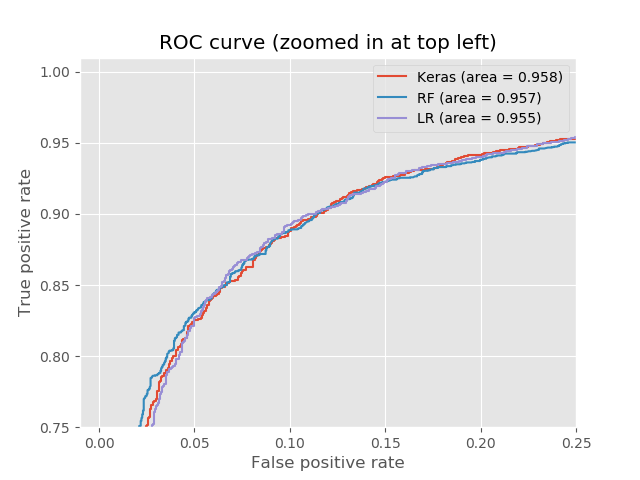
\includegraphics[scale=0.55]{../figures/ROC_zoom.png}
        \caption{PR Curve}
        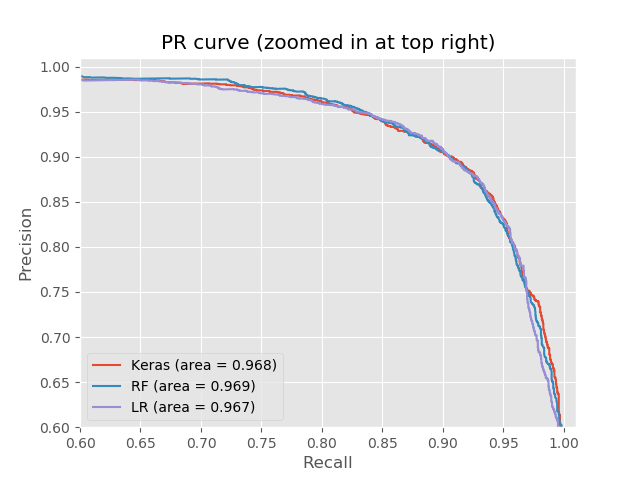
\includegraphics[scale=0.55]{../figures/PR_zoom.png}
\end{figure}

ANN performed slightly better than the Logistic regression model; however, the difference is minimal. 

\section{Discussion}

This disussion for each stage in the pipeline is discussed below.

\subsection{Feature Selection}

Starting off with the Recursive Feature Elimination (RFE) while using linear Support Vector Classification (SVC), three of the lowest ranked features were the AP Connection Count, Electricity Demand, and the Day of the Week. Due to the nature of the RFE algorithm, the lowest ranked features were desired. The CO$_2$ level of room 2102 was also ranked relatively close to the  three best features. The next best ranked feature was the Outside Air CO$_2$ Average, but this feature has nothing to do with building vacancy so it could be safely disregarded.

The Chi-Squared test showed the highest feature significance for the same three features as RFE: AP Connection Count, Electricity Demand, and Day of the Week. The p-values for all features are extremely low from the lowest being 0 for AP connections to $8.919819E-200$ for electricity demand to the highest being 0.496 for the average outside CO$_2$ which ends up with a score of about 0.4, which is lower than all other scores, the closest being about 21 and the highest around 1500. The most significant features also have scores that are significantly higher than all of the CO$_2$ features, which are themselves close to each other score-wise. The result of the Chi-Square test is shown in Figure 3.

\begin{figure}[H]
        \caption{Chi-Square Result}
        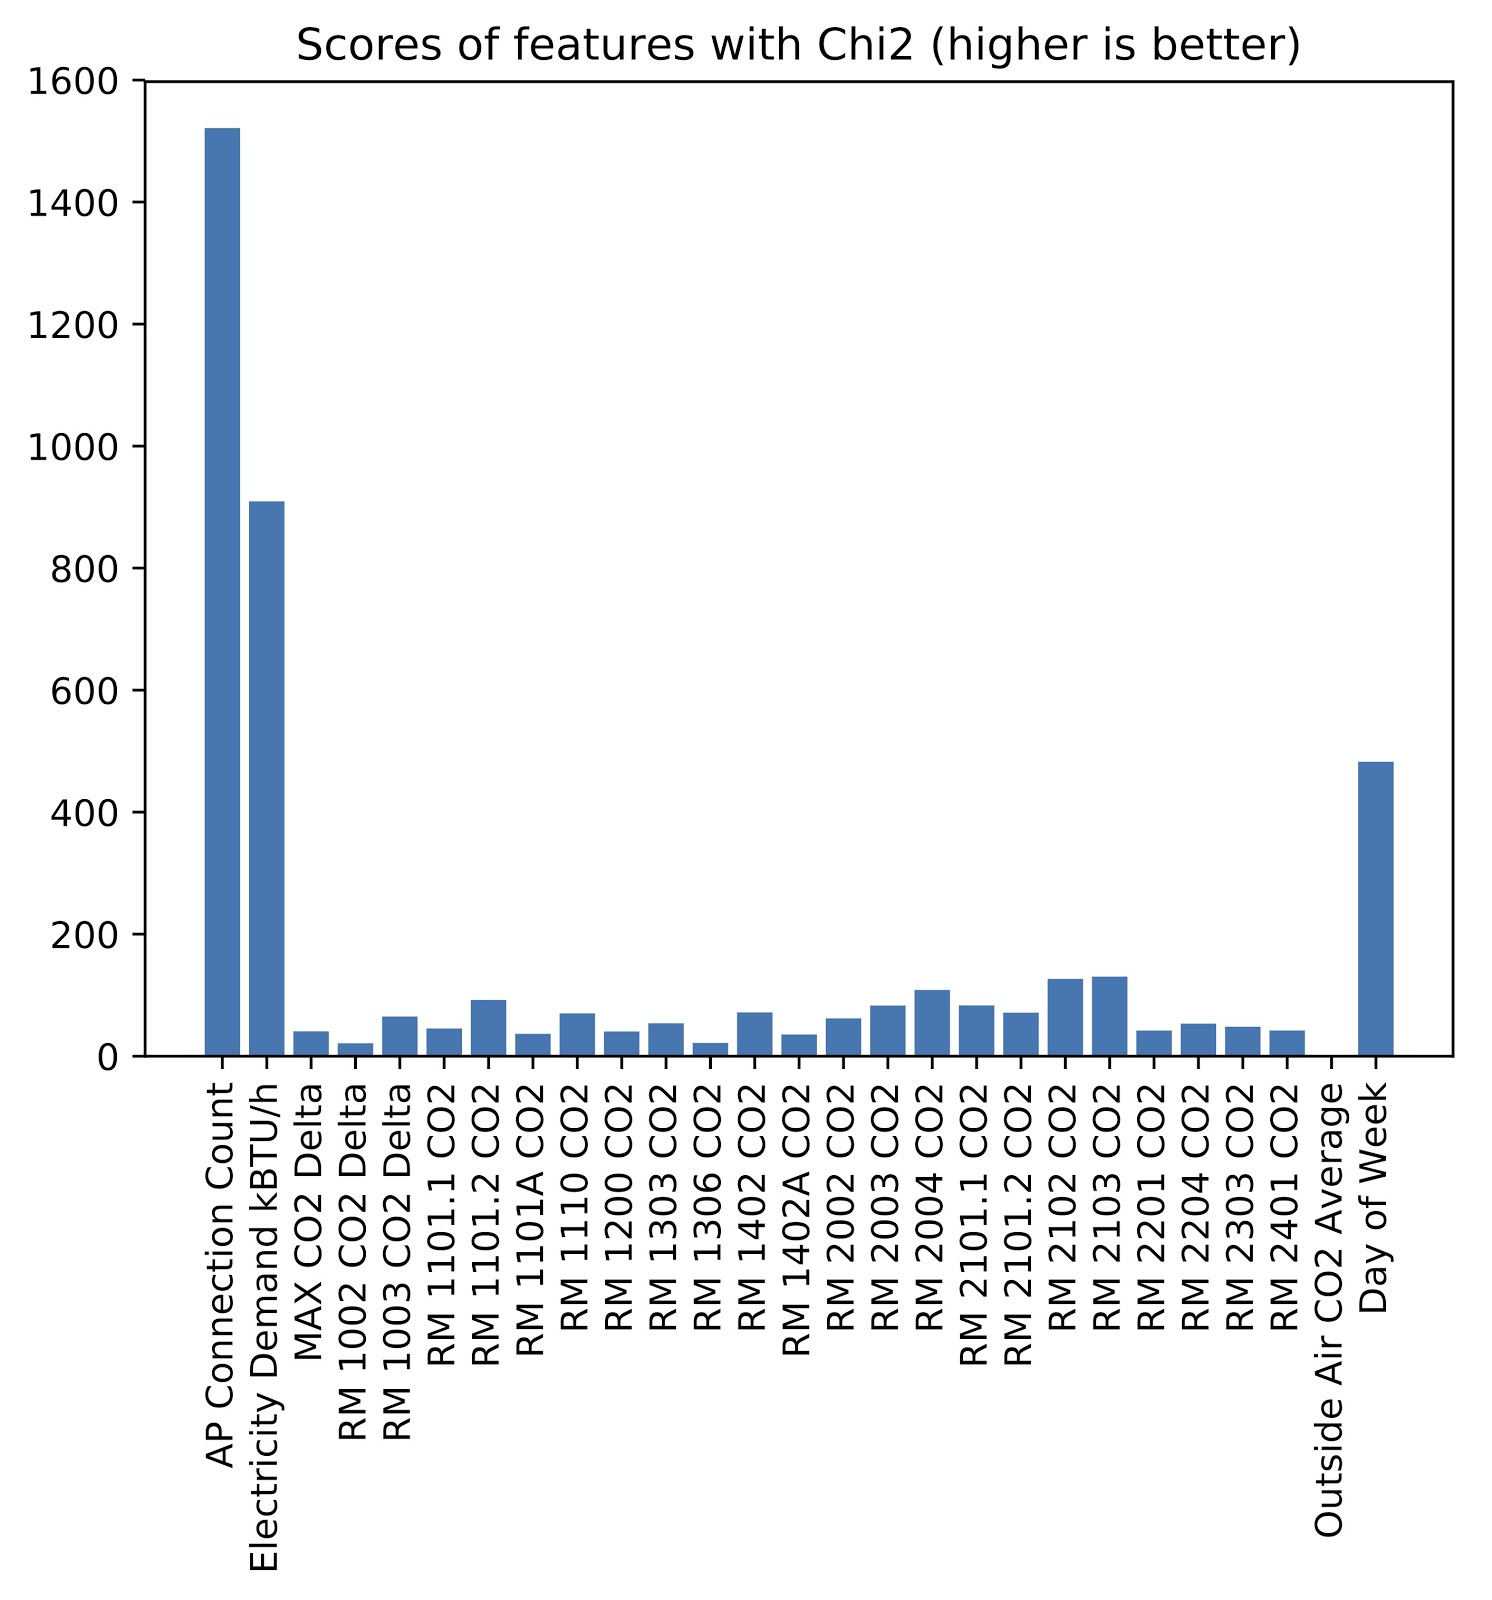
\includegraphics[scale=0.16]{../figures/chi2.jpg}
\end{figure}

The Extra Trees Classifier (ETC) gave very similar results to the Chi-Squared test with the same three peaks being above all of the other data. The AP connection count and electricity demand also have significantly higher scores than the day of the week which itself has the highest score from the rest of the other features. The ETC gives a closer result to the Chi-Squared test than the RFC. 

The RFC ranks the AP connection count and electricity demand the highest, except the day of the week has a score below about five other features of CO$_2$. The ETC can be more accurate than RFC which is evident in this case due to RFE and Chi-Squared being comparable with the ETC \cite{Geurts}. Pal \cite{Pal} also shows that decision-based tree methods are comparable to State Vector Machine (SVM) based classifiers, which is evident in the results between RFE and ETC since both assign highest significance to the same three features: AP Connection Count, Electricity Demand, and day of Week.
Comparing all of the results, the AP connection count and electricity demand were the features with the highest significance in all of the algorithms. The day of the week was marked as also being important in every algorithm except RFC.

By comparing all of the feature selection algorithms and the importance of each feature in each algorithm, all features that reference the CO$_2$ level of a room were removed. This was expected because the AP connection count and electricity demand can be directly matched to a person being inside a building whereas CO$_2$ experiences lag. With most people on campus having wireless devices and being connected to the campus wifi, as soon as someone walks into the the SCC, their wireless devices connect to the wifi indicating that the building is not vacant. Total electricity demand is a coarser measure of building vacancy because the same amount of lights can be on in a room regardless of head count. Similarly, the day of the week is representative because the building is mostly empty on weekends. While these features are immediately affected by a person’s presence, the CO$_2$ level exhibits a lag in the measurements. This is due to CO$_2$ being a gas and requiring time to diffuse through a room. This difference in response time between features cannot be intertwined due to a grey area where the CO$_2$ level cannot immediately match the AP connection count or electricity demand in determining building vacancy. Therefore, the CO$_2$ level features were removed from the dataset.

\subsection{ANN}
It was determined the ANN with ELU activation function for hidden layers, 9 hidden nodes per layer, 3 hidden layers, and a learning rate of 0.1 was the most optimal. It is worthwhile to note that this model only exhibits a 0.05\% increase in accuracy than the second best model. The small difference in performance between each model as well as the shuffling of data at runtime contribute to uncertainty that may be present in the results for each model.

A vast majority of the models trained in the grid search has a testing accuracy in 85\% to 89\% range, but a noteworthy number of models that had a sigmoid activation function did significantly worse in the 57\% range. It is worthwhile to note that models with the sigmoid activation function did still have the ability to score within the 85\% to 89\% testing accuracy range.

An alternative ANN setup consists of non-uniform number of nodes for each hidden layer was not examined. It will serve as a good direction for future experiments.

\subsection{Model Evaluation}

While testing accuracy is important, it is not the only indicator of the performance and effectiveness of a model. For the baseline logistic regression model and the best ANN model, the Receiver Operating Characteristic (ROC) curve and the Precision-Recall curve were plotted and the Area Under the Curve (AUC) was calculated for each graph. These are shown in Figure 1 \& 2. Both graphs were utilized because analyzing each graph alone may result in a misleading result. The ROC curve plots the True Positive Rate (TPR) against the False Positive Rate (FPR) with TPR on the y-axis and FPR on the x-axis. A perfect model would result in a curve that is horizontal line at $y=1$ which means that the model has no issues separating the classes and a random classifier would result in a line at $y=x$. The ROC curves for both models show an excellent degree of separation due to their shape and the AUC was 0.955 and 0.958 for logistic regression and ANN respectively. However, the shape of the ROC curve can be influenced by an imbalanced dataset. The Precision-Recall curve plots Precision against Recall with Precision on the y-axis and Recall on the x-axis. A perfect model would result in a curve that is a horizontal line at $y=1$ which shows that the model can separate the two classes with no overlap and a random classifier would result in a horizontal line at $y = \frac{\# of positive}{\# of positive + \# of negative}$. The Precision-Recall curves for both models confirm the results of the ROC graph and show that both models are very effective. The AUC was 0.967 for logistic regression and 0.968 for the ANN model. These graphs show that both models had excellent performance but logistic regression is much quicker and performs identically for this dataset. 

\section{CONCLUSION}

The objective of this report is to address the concern that an excessive amount of power is consumed during hours of vacancy in buildings. The report outlines a method of detecting vacancy via building data gathered by sensor outputs. Sample data from the UC Davis Student Community Center was used to test and train predictive models composed of logistic regression and an artificial neural network. Future work involves obtaining a similar data set for a large number of buildings, which would allow for clustering of buildings according to their occupancy schedules. A model could then be built for each of these clusters, which is expected to yield more generalizable results. To further improve upon this approach, the configuration of sensors should be optimized such that faulty sensors are repaired and sensors are placed in areas that can accurately collect the data of a room. New types of sensors, such as microphones and motion detectors could also be added to rooms to diversify the collection of data, allowing for more accurate measurements of vacancy of buildings. This approach is an application of existing machine learning methods, showcasing the benefits and uses of artificial neural networks and regression.  It reinforces the idea that machine learning can be utilized for a wide variety of improvements.

\addtolength{\textheight}{-12cm}   % This command serves to balance the column lengths
                                  % on the last page of the document manually. It shortens
                                  % the textheight of the last page by a suitable amount.
                                  % This command does not take effect until the next page
                                  % so it should come on the page before the last. Make
                                  % sure that you do not shorten the textheight too much.

%%%%%%%%%%%%%%%%%%%%%%%%%%%%%%%%%%%%%%%%%%%%%%%%%%%%%%%%%%%%%%%%%%%%%%%%%%%%%%%%



%%%%%%%%%%%%%%%%%%%%%%%%%%%%%%%%%%%%%%%%%%%%%%%%%%%%%%%%%%%%%%%%%%%%%%%%%%%%%%%%



%%%%%%%%%%%%%%%%%%%%%%%%%%%%%%%%%%%%%%%%%%%%%%%%%%%%%%%%%%%%%%%%%%%%%%%%%%%%%%%%

\begin{thebibliography}{99}

\bibitem{Perez-Lombard} Pérez-Lombard, L., Ortiz, J., Pout, C., A review on buildings energy consumption information. Energy and Buildings, 40, pp 394-398, 2008.
\bibitem{Casillas} Casillas, A., O{\' R}iordan, V., Garcia, J., Putting Vacant Buildings to Sleep. TS. Private Collection at University of California, Davis, June 2018.
\bibitem{Petersen} Petersen, S. et al., Establishing an image-based ground truth for validation of sensor data-based room occupancy detection. Energy and Buildings, 130, pp 787–793, 2016.
\bibitem{Viola} Viola, P., Jones, M., Rapid object detection using a boosted cascade of simple features. Proceedings of the 2001 IEEE Computer Society Conference on Computer Vision and Pattern Recognition. CVPR 2001, 1, I511-I518, 2001. 
\bibitem{Pedregosa} Pedregosa et al., Scikit-learn: Machine Learning in Python. JMLR 12, pp. 2825-2830, 2011.
\bibitem{LIBSVM} Chih-Chung Chang, Chih-Jen Lin, LIBSVM: A library for support vector machines. ACM Trans. Intell. Syst. Technol. 2, 3, Article 27, 27 pages, May 2011.
\bibitem{McHugh} McHugh, M.L., The Chi-square test of independence. Biochemia Medica, 23:2, pp 143-149, 2013.
\bibitem{Geurts} Geurts, P., Ernst, D., Wehenkel, L., Extremely randomized trees. Mach Learn, 63:1, pp 3-42, Apr. 2006.
\bibitem{Dreiseitl} Dreiseitl S, Osl M, Scheibb{\"o}ck C, Binder M., Outlier detection with one-class SVMs: An application to Melanoma Prognosis. AMIA Annu Symp Proc., 172-6, Nov., 2010.
\bibitem{Keras} Chollet, Fran{\c c}ois, Keras: The python deep learning library. Astrophysics Source Code Library, 2018.
\bibitem{Google} Google Brain Team Developers. “TensorFlow.” Apache 2.0 open source license, 2018.
\bibitem{Bottou} Bottou, L{\' e}on, Large-scale machine learning with stochastic gradient descent. Proceedings of COMPSTAT'2010: Physica-Verlag HD, 177-186, 2010.
\bibitem{Pal} Pal, M., Random forest classifier for remote sensing classification. International Journal of Remote Sensing, 26:1, pp 217-222, 2005.




\end{thebibliography}

\section{Contributions}

\subsection*{Benjamen Neduva}
        \begin{itemize}
                \item Initial feature analysis
                \item Report outline
        \end{itemize}

\subsection*{Calvin Cramer}
        \begin{itemize}
                \item ANN
                \item Grid search
                \item Normalization
        \end{itemize}

\subsection*{Lionel Quiambao}
        \begin{itemize}
                \item ANN
        \end{itemize}

\subsection*{Lisa Slaughter}
        \begin{itemize}
                \item Data acquisition
                \item Logistic Regression
                \item Project management
        \end{itemize}

\subsection*{Max Nedorezov}
        \begin{itemize}
                \item Feature selection
                \item Project scoping
        \end{itemize}

\subsection*{Richard Li}
        \begin{itemize}
                \item Report finalization
        \end{itemize}

\subsection*{Ryan Gosiaco}
        \begin{itemize}
                \item Initial feature analysis
                \item Model evaluation
        \end{itemize}

\subsection*{Victoria Salova}
        \begin{itemize}
                \item Outlier detection
        \end{itemize}

\subsection*{Yasmin Sayeed}
        \begin{itemize}
                \item No contribution
        \end{itemize}

\end{document}